\documentclass[ngerman,11pt,a4paper,titlepage]{article}

\usepackage{graphicx}
\usepackage{url}
\usepackage{bbm}
\usepackage{esvect}
\usepackage{amsmath}
\usepackage{units}
\usepackage{wrapfig}
\usepackage[super]{cite}
\usepackage[german,ngerman]{babel}
\usepackage[utf8]{inputenc}
%\usepackage[T1]{fontenc}

\usepackage{color}
\usepackage{listings}
\lstset{
language=matlab,
basicstyle=\scriptsize,
numbers=left,
numberstyle=\tiny,
stepnumber=1,
numbersep=5pt,
backgroundcolor=\color{white},
showspaces=false,
showstringspaces=false,
showtabs=false,
frame=single,
tabsize=2,
captionpos=b,
breaklines=true,
breakatwhitespace=false,
escapeinside={\%}{)}
}

\renewcommand{\UrlFont}{\small\tt}

\title{\Huge{Projektbericht}\\
\Large{
Finite Elemente Methode auf einer\\
2-dimensionalen Helmholtz Gleichung}}
\author{Juri Chomé}
\date{\today}

\begin{document}
\maketitle

\begin{abstract}
  Wir betrachten die Maxwell-Gleichungen für das Elektromagnetische Feld in einem Mikrowellenherd und interessieren uns für die dritte Komponente des Elektrischen Feldes. Diese entspricht einer 2-dimensionalen Helmholtz Gleichung. Mit Hilfe der Finiten-Elemente-Methode geht es dann darum, die Lösung dieser Gleichung in \emph{Matlab} zu implementieren. Dazu muss zuerst die schwache Formulierung des Problems hergeleitet werden und die Steifigkeitsmatrix und die Massenmatrix aus den jeweiligen Bilinearformen berechnet werden. Gegeben ist eine Triangulierung eines Fisches und der restlichen Mikrowelle als Liste von Knoten mit Materialinformationen. Die Triangulierung kann verfeinert werden, und die Matrizen werden möglichst effizient berechnet und gelöst. Zuletzt wird der Realteil der Lösung gezeichnet.
\end{abstract}

\section{Formulierung des Problems}
\subsection{Die Ausgangslage}
Gegeben sind die Maxwell-Gleichungen auf $\Omega \subset \mathbbm R^3$ für das elektrische Feld $\mathbf E:\Omega \rightarrow \mathbbm C^3$ und das magnetische Feld $\mathbf H:\Omega \rightarrow \mathbbm C^3$:

\begin{align}
  \nabla \times \mathbf E &= -\mu \mathbf H_t \label{max1} \\
  \nabla \times \mathbf H &= \varepsilon \mathbf E_t + \sigma \mathbf E. \label{max2}
\end{align}

Hier entsprechen $\varepsilon$, $\sigma$ und $\mu$ der dielektrischen Leitfähigkeit, der Konduktivität und der Permeabilität und sind im Aufgabenblatt jeweils in der Luft und im Fisch konkret definiert. Vorgegeben wird zudem, dass die Lösung zeit-harmonisch ist:
\begin{align*}
  \mathbf E = \mathbf E(x,y,z) e^{i\omega t} \text{ und } \mathbf H = \mathbf H(x,y,z) e^{i\omega t}.
\end{align*}

\subsection{Herleitung}
Mit dem Kreuzprodukt und der Periodizität der Gleichungen erhalten wir
\begin{align*}
  (\nabla \times \mathbf E) =
  \begin{pmatrix}
    \partial_y \mathbf E_3 - \partial_z \mathbf E_2 \\
    \partial_z \mathbf E_1 - \partial_x \mathbf E_3 \\
    \partial_x \mathbf E_2 - \partial_y \mathbf E_1
  \end{pmatrix}
  = (\nabla \times \mathbf E) \cdot e^{i\omega t} 
\end{align*}
auf der linken Seite und
\begin{align*}
  -\mu \mathbf H_t = -(i\omega)\mu \mathbf H \cdot e^{i\omega t} 
\end{align*}
auf der rechten Seite. Also lautet \eqref{max1} nun
\begin{align*}
  \nabla \times \mathbf E = -i\omega \mu \mathbf H.
\end{align*}
Das Gleiche machen wir für \eqref{max2} und erhalten so
\begin{align*}
  (\nabla \times \mathbf H) \cdot e^{i\omega t} = (\varepsilon i \omega + \sigma)\mathbf E \cdot e^{i\omega t}.
\end{align*}
Also lautet unser Gleichungssystem nun
\begin{align*}
  \nabla \times \mathbf E &= -i\omega \mu \mathbf H \\
  \nabla \times \mathbf H &= i\omega \tilde \varepsilon \mathbf E && \text{in } \Omega \subset \mathbbm R^3
\end{align*}
für $\tilde \varepsilon := \varepsilon + \frac{\sigma}{i\omega}$.
Als zweite Annahme wird angegeben, dass $\partial_z \mathbf E = \partial_z \mathbf H = \vv 0$ ist. Also gilt mit dem Kreuzprodukt jetzt
\begin{align}
  (\nabla \times \mathbf E) =
  \begin{pmatrix}
    \partial_y \mathbf E_3\\
    - \partial_x \mathbf E_3 \\
    \partial_x \mathbf E_2 - \partial_y \mathbf E_1
  \end{pmatrix}
  = -i\omega \mu \mathbf H
  \label{neu1}
\end{align}
und
\begin{align}
  (\nabla \times \mathbf H) =
  \begin{pmatrix}
    \partial_y \mathbf H_3\\
    - \partial_x \mathbf H_3 \\
    \partial_x \mathbf H_2 - \partial_y \mathbf H_1
  \end{pmatrix}
  = i\omega \tilde \varepsilon \mathbf E.
  \label{neu2}
\end{align}
%
Aus \eqref{neu1} und \eqref{neu2} ergeben sich folgende Identitäten:
\begin{align}
  - \partial_y \mathbf E_3 &= i\omega \mu \mathbf H_1 \label{neua} \\
  \partial_x \mathbf E_3 &= i\omega \mu \mathbf H_2 \label{neub} \\
  \partial_x \mathbf H_2 - \partial_y \mathbf H_1 &= i\omega \tilde \varepsilon \mathbf E_3. \label{neuc}
\end{align}
%
Setze \eqref{neua} und \eqref{neub} in \eqref{neuc} ein und multipliziere mit $i\omega \mu$:
\begin{align*}
  \partial_x^2 \mathbf E_3 + \partial_y^2 \mathbf E_3 &= -\omega^2\mu \tilde \varepsilon \mathbf E_3 \\
  \iff \Delta \mathbf E_3 + \omega^2\mu \tilde \varepsilon \mathbf E_3 &= 0.
\end{align*}
Also stehen wir nun vor der 2-dimensionalen Helmholtz-Gleichung
\begin{align}
  \Delta u + (\omega^2\mu \tilde \varepsilon) u &= 0 && \text{ in } \Omega \subset \mathbbm R^2 \label{helm} \\
  u &= g && \text{ auf } \partial \Omega. \label{rb}
\end{align}
%Falls $\omega = 0$ ist, dann

\section{Schwache Formulierung}
Multipliziere wie immer \eqref{helm} mit einer Testfunktion $v\in H_0^1(\Omega)$, integriere und nutze die Greensche Formeln:
\begin{align*}
  \int_\Omega \Delta u \cdot v + \omega^2\mu \tilde \varepsilon \int_\Omega u\cdot v &= 0 \\
  \iff - \underbrace{\int_\Omega \nabla u \cdot \nabla v}_{=:\text{ }a_1(u,v)} +
    \underbrace{\int_{\partial \Omega} v\cdot \frac{\partial u}{\partial \vv N}}_{\equiv 0\text{, da } v \equiv 0 \text{ auf } \partial \Omega}
    + \omega^2\mu \tilde \varepsilon \underbrace{\int_\Omega u\cdot v}_{=:\text{ }a_2(u,v)} &= 0.
\end{align*}
Wir erhalten also die Gleichung
\begin{align*}
  a(u,v) = a_1(u,v) - \omega^2\mu \tilde \varepsilon \cdot a_2(u,v) = 0
\end{align*}
und somit die schwache Formulierung: "`Suche $u\in H^1(\Omega )$, so dass $a(u,v)=0$ $\forall v \in H_0^1(\Omega)$ und $u\equiv g$ auf $\partial\Omega$"'.

\section{Implementierung}
\subsection{Methode}
Wir benutzen eine lineare Finite-Elemente Methode auf Dreiecken welche die Eckpunkte nutzt. Dazu ist eine Liste $N$ von Knotenpunkten gegeben (x und y Koordinaten) und eine Liste von Dreiecken $T$, die sich auf $N$ beruft um die Eckpunkte der Dreiecke zu definieren. Zusätzlich enthält $T$ noch drei binärwertige Kolonnen, die angeben, ob sich die dazugehörige Kante auf dem Rand befindet oder nicht. Zuletzt enthält ein Vektor $P$ für jedes Dreieck die dazugehörigen Materialkonstante $\mu(\varepsilon + \frac{\sigma}{i\omega})$, in unserem Fall entweder die für den Fisch oder die in der Luft.

\paragraph{}In Abbildung \ref{drei} sieht man als Beispiel vier Dreiecke, von denen drei eine Kante am Rand besitzen (fett gedruckte Linie) und die insgesamt sechs verschiedene Punkte benötigen. Die Listen $N$ und $T$ sehen in dem Fall folgendermassen aus:

\begin{lstlisting}
N =             T =

  0    0        1  4  6   1  0  1
  1    0        4  5  6   0  0  0
  0    1        4  2  5   1  0  0
0.5    0        6  5  3   0  0  1
0.5  0.5
  0  0.5
\end{lstlisting}

\begin{figure}[h]
  \begin{center}
    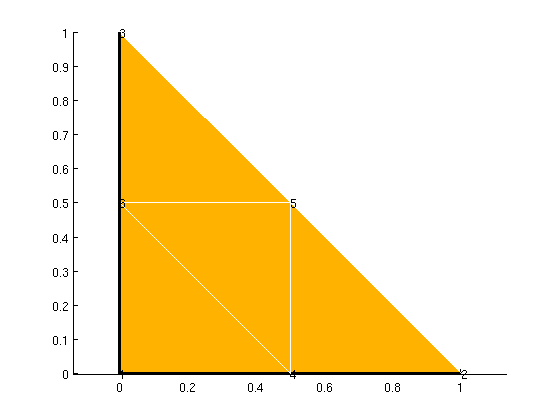
\includegraphics[scale=0.75]{pics/dreieck.png}
  \end{center}
  \caption{Ein 4-fach unterteiltes Dreieck}
  \label{drei}
\end{figure}

\subsection{Gitterverfeinerung}
Die Prozedur der Gitterverfeinerung erhält die Listen der Knotenpunkte $N$, die der Dreiecke $T$ (inklusive Randinformationen) und die der dazugehörigen Materialkonstanten $P$. Das Ziel ist es ein gegebenes Gitter zu verfeinern indem jedes Dreieck in vier kleinere unterteilt wird und die dazu nötigen Knotenpunkte zu berechnen. Um die neue Liste der Punkte zu erstellen muss allerdings vermieden werden, Punkte doppelt zu definieren. Dazu wird eine einfache \emph{for}-Schleife über die drei möglicherweise redundanten Punkte erstellt. In pseudo-Matlabcode sieht dies dann folgendermassen aus:

\begin{lstlisting}
for i=1:size(T,1),
  uebernimm die gueltigen alten Eckpunkte;
  uebernimm Materialkonstanten;
  
  punkte_neu(1,1)=(%$x_1$)+%$x_2$))/2; punkte_neu(1,2)=(%$y_1$)+%$y_2$))/2;
  punkte_neu(2,1)=(%$x_3$)+%$x_2$))/2; punkte_neu(2,2)=(%$y_3$)+%$y_2$))/2;
  punkte_neu(3,1)=(%$x_1$)+%$x_3$))/2; punkte_neu(3,2)=(%$y_1$)+%$y_3$))/2;

  for j=1:3
    dupe=find(ismember(Nr,punkte_neu(j,:),'rows'));
    if isempty(dupe)
      Nr(size(N,1)+1,:)=punkte_neu(j,:);
      uebernimm die neuen Punkte;
    else
      uebernimm die alten Punkte;
    end
  end
end
\end{lstlisting}
Als Beispiel sieht man das Einheitsquadrat nach dreifacher Verfeinerung in Abbildung \ref{quad3}.
\begin{figure}[h]
  \begin{center}
    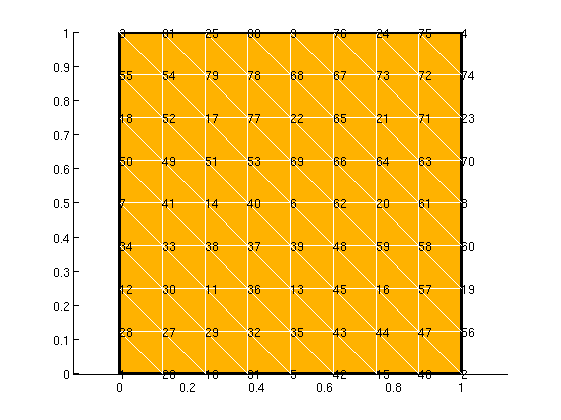
\includegraphics[scale=0.75]{pics/quad3.png}
  \end{center}
  \caption{Das Gitter des dreifach verfeinerten Einheitsquadrates}
  \label{quad3}
\end{figure}

\subsection{Matrizen}
Um nicht für jedes Element die Basisfunktionen neu definieren zu müssen, wird eine Transformation auf das Referenzdreieck $\hat K$ vollzogen. Die Basisfunktionen lauten dort
\begin{align*}
  \varphi_1(\xi_1,\xi_2) &= 1-\xi_1-\xi_2 \\
  \varphi_2(\xi_1,\xi_2) &= \xi_1 \\
  \varphi_3(\xi_1,\xi_2) &= \xi_2.
\end{align*}

Für die drei Eckpunkte $P_1$, $P_2$, $P_3$ von $K$ lautet die affine Transformation $F_K := P_1+(P_2-P_1)\xi_1 +(P_3-P_1)\xi_2$.

\subsubsection*{Elementsteifigkeitsmatrix}
Mit der Herleitung die wir in der Vorlesung gesehen haben, lässt sich für $a_1$ die Elementsteifigkeitsmatrix berechnen mit
\begin{align*}
  A_e=\frac{1}{2}|\det J |\cdot D D'
\end{align*}
wobei
\begin{align*}
  J:=
  \begin{pmatrix}
    x_2 - x_1 & x_3 - x_1 \\
    y_2 - y_1 & y_3 - y_1
  \end{pmatrix}
\end{align*}
und
\begin{align*}
  D:=
  \begin{pmatrix}
    -1 & -1\\
    1 & 0\\
    0 & 1
  \end{pmatrix}
  \cdot J^{-1}.
\end{align*}
In \emph{Matlab} sieht das dann folgendermassen aus:
\begin{lstlisting}
J=[N(T(el,2),1)-N(T(el,1),1) N(T(el,3),1)-N(T(el,1),1);
   N(T(el,2),2)-N(T(el,1),2) N(T(el,3),2)-N(T(el,1),2)];

D=[-ones(1,2);eye(2)]/J;

Ae=1/2*abs(det(J))*D*D';
\end{lstlisting}

\subsubsection*{Elementmassenmatrix}
Auf $\hat K$ lauten die Einträge
\begin{align*}
  a_2(i,j) := \int_{\hat K} \varphi_i \varphi_j && i,j=1,2,3.
\end{align*}
Das Resultat ist $\nicefrac{1}{12}$ auf den Diagonalen und $\nicefrac{1}{24}$ sonst. Damit berechnen wir für jedes Element die Elementmassenmatrix
\begin{align*}
  M_e = |\det{J}| \cdot a_2(i,j).
\end{align*}
%wobei $J_K$ aus der affinen Transformation $F_K$ hergeleitet wird. Eine Möglichkeit ist
%\begin{align*}
%  J_K =
%  \begin{pmatrix}
%    1 & x_1 & y_1 \\
%    1 & x_2 & y_2 \\
%    1 & x_3 & y_3
%  \end{pmatrix}.
%\end{align*}
Der \emph{Matlab} Code ist somit
\begin{lstlisting}
J=[N(T(el,2),1)-N(T(el,1),1) N(T(el,3),1)-N(T(el,1),1);
   N(T(el,2),2)-N(T(el,1),2) N(T(el,3),2)-N(T(el,1),2)];

Me=[1/12 1/24 1/24;
    1/24 1/12 1/24;
    1/24 1/24 1/12];

Me=abs(det(J))*Me;
\end{lstlisting}

\subsubsection*{Assemblierung}
Die Assemblierungsroutine läuft über alle Dreiecke, berechnet die beiden dazugehörigen Elementmatrizen und multipliziert $M_e$ mit der entsprechenden Materialkonstante aus $P$. Um die Matrizen zusammenzustellen wird im Prinzip nur für jedes Element die Elementmatrix dazu addiert:
\begin{lstlisting}
k=T(i,1:3);
A(k,k)=A(k,k)-Ae;
M(k,k)=M(k,k)+Me;
\end{lstlisting}
Das negative Vorzeichen der Steifigkeitsmatrix kommt von dem Minus und von der homogenität der Gleichung. Schlussendlich müssen noch die Randbedingung \eqref{rb} beachtet werden. Man macht also eine Liste die prüft, ob ein Dreieck einen Randpunkt besitzt und erstellt eine Schleife über alle Knotenpunkte um die Matrizen zu modifizieren:
\begin{lstlisting}
n=size(T,1);
m=size(N,1);
for i=1:n,
  bn(T(i,1))=bn(T(i,1)) | T(i,4) | T(i,6);
  bn(T(i,2))=bn(T(i,2)) | T(i,4) | T(i,5);
  bn(T(i,3))=bn(T(i,3)) | T(i,5) | T(i,6);
end
for j=1:m
  if bn(j)==1
    A(j,:)=0;
    A(j,j)= 1;
    M(j,:)=0;
    b(j)=feval(g,N(j,1),N(j,2));
  end
end
\end{lstlisting}

\subsection{Ergebnisse}
\subsubsection*{Testproblem}
Mit $\omega=0$ kann man die Implementierung testen, da die Gleichung dann ein Poisson-Problem ist. Gibt man sich die Randbedingung $g:=x+y$, dann lautet die exakte Lösung auf dem Einheitsquadrat ganz einfach $u(x,y)=x+y$, da $\Delta u = 0$ ergibt. In Abbildung \ref{poiss} kann man sich davon überzeugen, dass \emph{mainPoisson.m} tatsächlich genau diese Lösung ausspuckt. Die Gitterverfeinerung ist hier viermal auf das Einheitsquadrat angewendet worden.
\begin{figure}[h]
  \begin{center}
    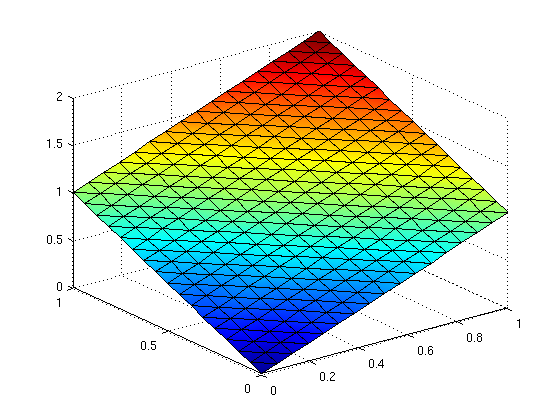
\includegraphics[scale=0.75]{pics/poisson.png}
  \end{center}
  \caption{Die Lösung der Poisson Gleichung mit Matlab}
  \label{poiss}
\end{figure}

\subsubsection*{Fisch}
Die Randbedingung $g$ ist in diesem Fall gegeben durch
\begin{align*}
  g(x,y) &=100 \text{ auf dem Intervall } 0,5 \times [0,1;0,2]\\
  g(x,y) &=0 \text{ sonst}.
\end{align*}
Die Konstanten lauten
\begin{align*}
  \mu_F &= 2\pi\cdot 10^{-7},\\
  \varepsilon_F &= 6,44\cdot 10^{-10},\\
  \sigma_F &= 3\cdot 10^{-11}\\
  \mu_L &= 2\pi\cdot 10^{-7},\\
  \varepsilon_L &= 8,85\cdot 10^{-12},\\
  \sigma_L &= 0
\end{align*}
jeweils auf dem Fisch und in der Luft.

\paragraph{}Schliesslich lässt man die Routinen auf den Fisch in der Mikrowelle los und erhält nach vier Gitterverfeinerungen als Lösung die reellen Komponenten des elektrischen Feldes, die man in Abbildung \ref{res} sehen kann, einmal nur auf dem Fisch, einmal aus isometrischer dreiviertel-Ansicht, und einmal von oben.
\begin{figure}[h]
  \begin{center}
    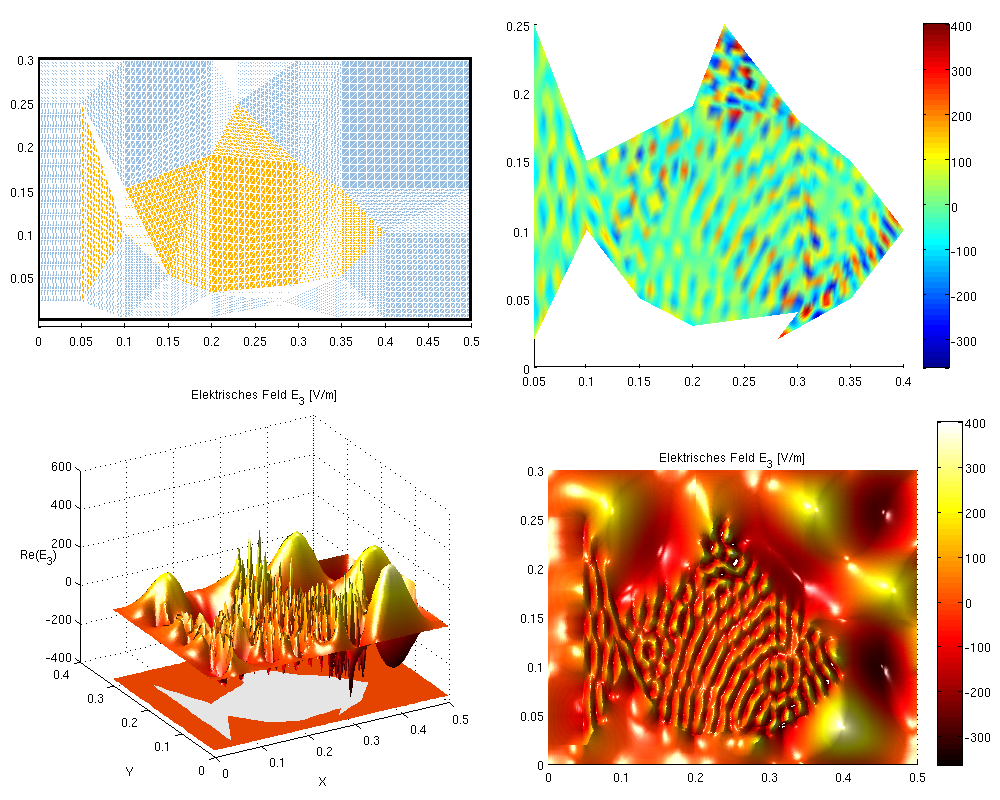
\includegraphics[scale=0.5]{pics/end_result_all.png}
  \end{center}
  \caption{Das Resultat nach 4 Verfeinerungen mit dem dazugehörigen Gitter}
  \label{res}
\end{figure}

\end{document}
